\section{Natural Clouds}
Clouds are a substantial part of Earth's weather. They provide shade from the glistening sun on hot days and reflect the heat at night, keeping the ground warmer.
For a layman, clouds are comprehensible and useful indicators for telling the weather.
If they are dark and low-hanging, they usually bring rain.
If they are puffy and scarce, they predict fair weather ahead.

\subsection{Convection}
\label{section:clouds:convection}
In meteorology, \gls{convection} describes the event of atmospheric motions in the vertical direction.
Hot air rises from Earth's surface in form of bubbles, which are called \emph{\gls{thermal}s}.
As the \gls{altitude} increases, the thermals cool down. At some point, the warm air mixes with the surrounding colder air, after which its moisture condenses and starts forming clouds \cite{weather:convection}.

\begin{figure}[H]
    \centering
    \begin{tikzpicture}[scale=1.2]
        \tikzset{edge/.style = {-{Latex[length=3mm]},shorten >= -4pt}}
        \tikzset{shortedge/.style = {-{Latex[length=3mm]},shorten <=-4pt,shorten >= -4pt}}
        \tikzset{line/.style = {shorten >=-4pt}}
        \tikzset{icon/.style = {font=\Large}}

        % clouds
        \node[text width=2cm] (cloud) at (4.0, 3.0) {cloud starts \phantom{x} forming};
        \node[cloud, rotate=0, cloud puffs=15.7, cloud, minimum width=3.5cm, minimum height=2.2cm, align=center, draw] (cloud) at (cloud) {};

        % thermal
        \node (t1) at (4, 0.5) {};
        \node[red] (t1t) at (5.9, 1.2) {thermals rising upwards};
        \node (t2) at (4, 1.8) {};
        \draw[red,edge] (t1) -- (t2);

        % cold air
        \node (l1) at (3, 4.0) {};
        \node (l2) at (2, 3.0) {};
        \node (r1) at (5, 4.0) {};
        \node (r2) at (6, 3.0) {};
        \node[cyan] (r2t) at (6.8, 3.8) {sinking air};
        \draw[cyan,edge] (l1) to [out=180,in=90] (l2);
        \draw[cyan,edge] (r1) to [out=0,in=90] (r2);

        \end{tikzpicture}
    \captionof{figure}{Lifting by convection.}
    \label{img:tikz:convection}
\end{figure}

% \noindent
% A \gls{thermal} does not have to rise naturally. It can also be pushed upwards by a cold front.

% \begin{figure}[H]
%     \centering
%     \begin{minipage}{0.47\linewidth}
%         \begin{tikzpicture}
%             \tikzset{edge/.style = {-{Latex[length=3mm]},shorten >= -4pt}}
%             \tikzset{shortedge/.style = {-{Latex[length=3mm]},shorten <=-4pt,shorten >= -4pt}}
%             \tikzset{line/.style = {shorten >=-4pt}}
%             \tikzset{icon/.style = {font=\Large}}

%             % clouds
%             \node[text width=2cm] (cloud) at (4.0, 3.0) {cloud starts \phantom{x} forming};
%             \node[cloud, rotate=0, cloud puffs=15.7, cloud, minimum width=3.5cm, minimum height=2.2cm, align=center, draw] (cloud) at (cloud) {};

%             % thermal
%             \node (t1) at (4, 0.5) {};
%             \node[red] (t1t) at (5.9, 1.2) {thermals rising upwards};
%             \node (t2) at (4, 1.8) {};
%             \draw[red,edge] (t1) -- (t2);

%             % cold air
%             \node (l1) at (3, 4.0) {};
%             \node (l2) at (2, 3.0) {};
%             \node (r1) at (5, 4.0) {};
%             \node (r2) at (6, 3.0) {};
%             \node[cyan] (r2t) at (6.8, 3.8) {sinking air};
%             \draw[cyan,edge] (l1) to [out=180,in=90] (l2);
%             \draw[cyan,edge] (r1) to [out=0,in=90] (r2);
%         \end{tikzpicture}
%         \captionof{figure}{Convection: Cold front approaching.}
%         \label{img:tikz:convection:cold1}
%     \end{minipage}        
%     \hfill
%     \begin{minipage}{0.47\linewidth}
%         \begin{tikzpicture}
%             \tikzset{edge/.style = {-{Latex[length=3mm]},shorten >= -4pt}}
%             \tikzset{shortedge/.style = {-{Latex[length=3mm]},shorten <=-4pt,shorten >= -4pt}}
%             \tikzset{line/.style = {shorten >=-4pt}}
%             \tikzset{icon/.style = {font=\Large}}

%             % clouds
%             \node[text width=2cm] (cloud) at (4.0, 3.0) {cloud starts \phantom{x} forming};
%             \node[cloud, rotate=0, cloud puffs=15.7, cloud, minimum width=3.5cm, minimum height=2.2cm, align=center, draw] (cloud) at (cloud) {};

%             % thermal
%             \node (t1) at (4, 0.5) {};
%             \node[red] (t1t) at (5.9, 1.2) {thermals rising upwards};
%             \node (t2) at (4, 1.8) {};
%             \draw[red,edge] (t1) -- (t2);

%             % cold air
%             \node (l1) at (3, 4.0) {};
%             \node (l2) at (2, 3.0) {};
%             \node (r1) at (5, 4.0) {};
%             \node (r2) at (6, 3.0) {};
%             \node[cyan] (r2t) at (6.8, 3.8) {sinking air};
%             \draw[cyan,edge] (l1) to [out=180,in=90] (l2);
%             \draw[cyan,edge] (r1) to [out=0,in=90] (r2);
%         \end{tikzpicture}
%         \captionof{figure}{Convection: Cold front pushing creating thermals.}
%         \label{img:tikz:convection:cold2}       
%     \end{minipage}
% \end{figure}

\subsection{Classifications}
In order to create a \gls{wrs} that is able to display many different cloudscapes, all types of clouds have to be understood first.
The \gls{wmo} describes ten distinct cloud classifications. For each of those, there are further subtypes. For simplicity, those subtypes will be disregarded in this project.

\begin{figure}[H]
    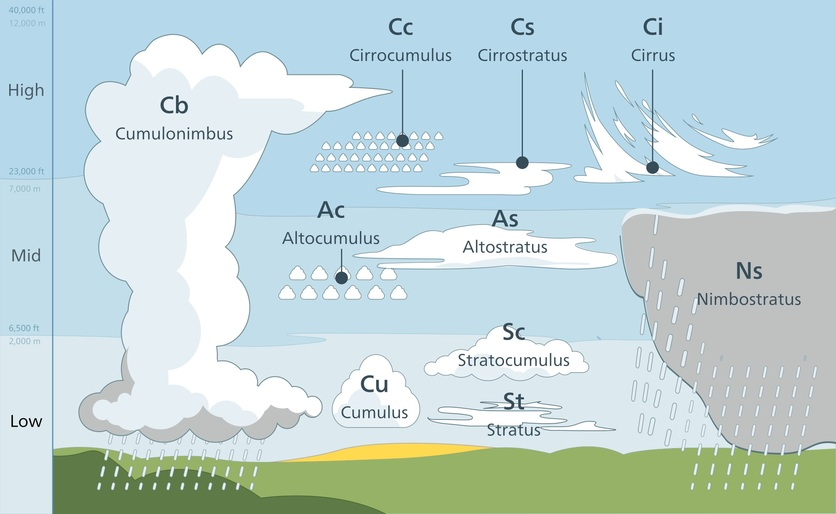
\includegraphics[width=\linewidth]{clouds-types.jpg}
    \captionof{figure}{Distinct classifications of cloudshapes in the troposphere \protect\cite{cloudtypes:wiki}.}
    \label{img:ui:mockup:live}
\end{figure}

\noindent
This graphic above provides and excellent overview of all distinct cloud types.
Each type is depicted in its signature shape and marked with the scientific name and abbreviation.
Natural clouds are typically identified by two major factors: shape and \gls{altitude}.
The \gls{altitude}, which is the distance from sea level to the cloud, is further split into three categories "low", "mid" and "high".
This corresponds to the altitude at which the cloud usually forms, up to twelve kilometers above ground. 
\\
All of those clouds are formed in the troposphere, Earth's lowest atmospheric layer.
Certain clouds may occur in the stratospheric or even the mesospheric layer, but they are usually a rare sight. Therefore, those clouds will not be covered in this project.

% refs:
% https://www.countryfile.com/how-to/outdoor-skills/how-to-predict-the-weather-forecast-using-clouds/
% NASA how do clouds form: https://climatekids.nasa.gov/cloud-formation/#:~:text=Clouds%20are%20created%20when%20water,are%20floating%20in%20the%20air.&text=That%20means%20some%20of%20the,drifted%20away%20into%20the%20atmosphere.
% NASA: https://www.nasa.gov/audience/forstudents/k-4/stories/nasa-knows/what-are-clouds-k4.html

\pagebreak

\subsubsection{Cirrus}
\begin{wrapfigure}[10]{r}{6cm}
    \vspace{-\baselineskip}
    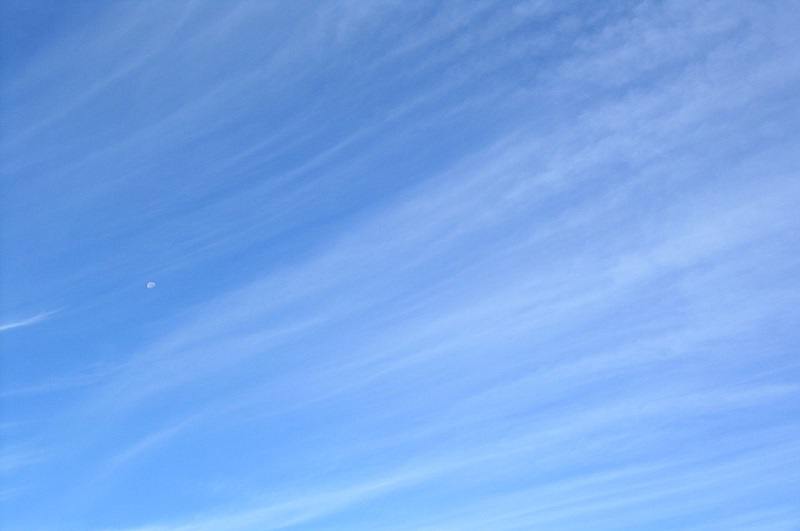
\includegraphics[width=6cm]{clouds/cirrus.jpg}
    \caption{Cirrus clouds \protect\cite{cloudtypes:wiki:cirrus}.}
    \label{img:clouds:cirrus}
\end{wrapfigure}
Cirrus clouds consist of thin, hair-like strands.
They fall into the "high" altitude group and mostly appear in a bright white color, although they may take on the colors of the sunset or sunrise.
Typically, they are formed when \gls{watervapor} undergoes \gls{desublimation}, the process in which gas turns into solid. This occurs when the \gls{watervapor} freezes rapidly at high altitudes, turning into ice crystals.
\\
\noindent
However, cirrus clouds can also form from air that flows outwards of thunderstorms.
\emptyline
\textbf{Interpretation:} Fair weather, but they might announce the arrival of warm front in 12-24 hours, which is often preceded by rain several hours in advance.
Even though cirrus clouds indicate \gls{precipitation}, they themselves do not produce rainfall \cite{predict:weather}.

\subsubsection{Cirrostratus}
\begin{wrapfigure}[10]{r}{6cm}
    \vspace{-\baselineskip}
    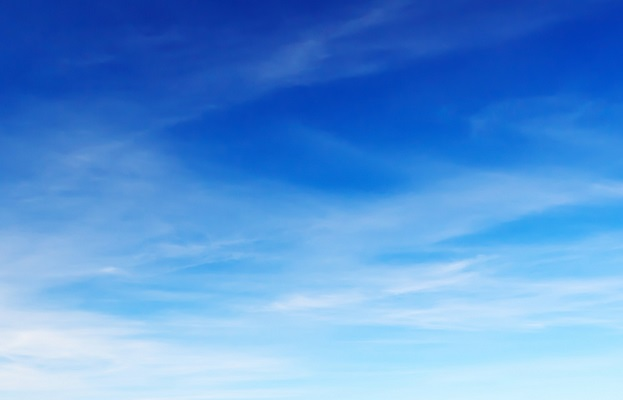
\includegraphics[width=6cm]{clouds/cirrostratus.jpg}
    \caption{Cirrostratus clouds \protect\cite{cloudtypes:wiki:cirrostratus}.}
    \label{img:clouds:cirrostratus}
\end{wrapfigure}
Cirrostratus clouds are similar to the cirrus clouds, only that they are even thinner.
Those clouds depict more of a veil than a single cloud shape.
They form under the same conditions as the cirrus clouds and can cover a massive area of the sky, spanning thousands of kilometers.
\\
\noindent
Cirrostratus clouds sometimes produce white rings or arcs of lights around the sun or the moon called the \emph{\gls{halophenomenon}}.
Sometimes, the cirrostratus clouds are so thin that the halo is the only way to tell if there are cirrostratus clouds.
\emptyline
\textbf{Interpretation:} Fair weather, but they indicate a warm front within one or two days, bringing \gls{precipitation} \cite{cloudtypes:meteoblue}.

\subsubsection{Cirrocumulus}
\begin{wrapfigure}[10]{r}{6cm}
    \vspace{-\baselineskip}
    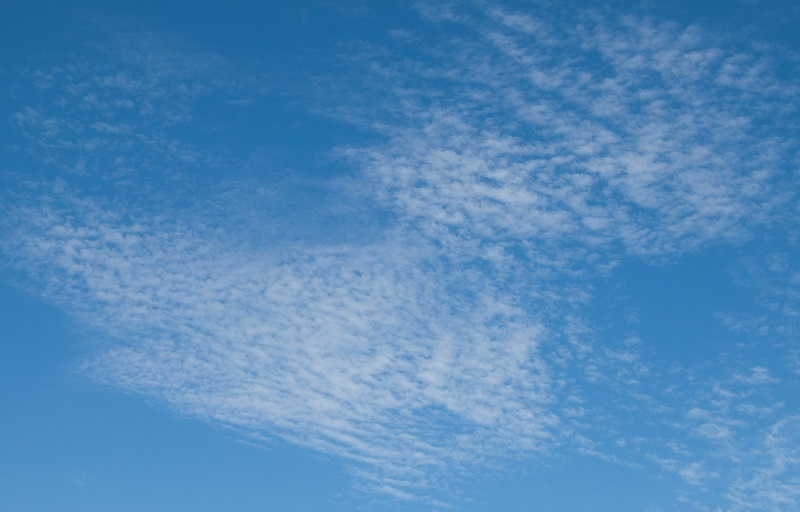
\includegraphics[width=6cm]{clouds/cirrocumulus.jpg}
    \caption{Cirrocumulus clouds \protect\cite{cloudtypes:wiki:cirrocumulus}.}
    \label{img:clouds:cirrocumulus}
\end{wrapfigure}
Similar to the other clouds of the cirrus-family, the cirrocumulus are composed of ice crystals and formed at high \gls{altitude}s.
They are made up of many small, white, puffy clouds called \emph{\gls{cloudlet}}s. Their wooly look give the cloud the name \emph{cumulus}.
\\
\noindent
Cirrocumulus clouds are realtively rare, as they are naturally only formed when a turbulent vertical current meets a cirrus cloud layer. The cirrus cloud then disperses into many \gls{cloudlet}s.
\emptyline
\textbf{Interpretation:} 
They do produce \gls{precipitation}, but it never reaches the surface, meaning that cirrocumulus clouds are typically associated with fair weather \cite{cloudtypes:meteoblue}.

\clearpage

\subsubsection{Altostratus}
\begin{wrapfigure}[10]{r}{6cm}
    \vspace{-\baselineskip}
    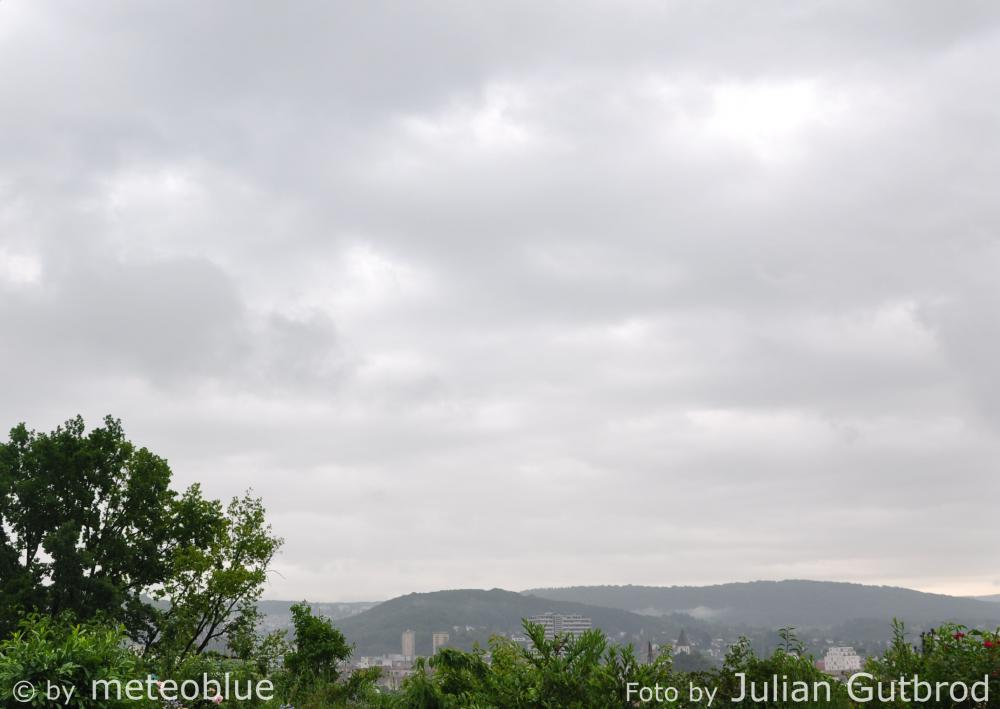
\includegraphics[width=6cm]{clouds/altostratus.jpg}
    \caption{Altostratus clouds \protect\cite{cloudtypes:meteoblue}.}
    \label{img:clouds:altostratus}
\end{wrapfigure}
The name for this grey, uniform sheet of clouds consists of the latin words \emph{alto} (height) and \emph{stratus} (layered), summing up their appearance accurately.
Altostratus clouds usually cover the whole sky and form a dull blanket of monocolored clouds with very few features.
The sun- or moonlight may shine through them, but will most likely not be strong enough to cast defined shadows.
\emptyline
\textbf{Interpretation:}
Altostratus clouds usually indicate \gls{precipitation}, even more so if they are are preceded by cirrus clouds.
If the \gls{precipitation} increases in persistence and intensity, the altostratus clouds will lower and thicken into nimbostratus clouds.


\subsubsection{Altocumulus}
\begin{wrapfigure}[10]{r}{6cm}
    \vspace{-\baselineskip}
    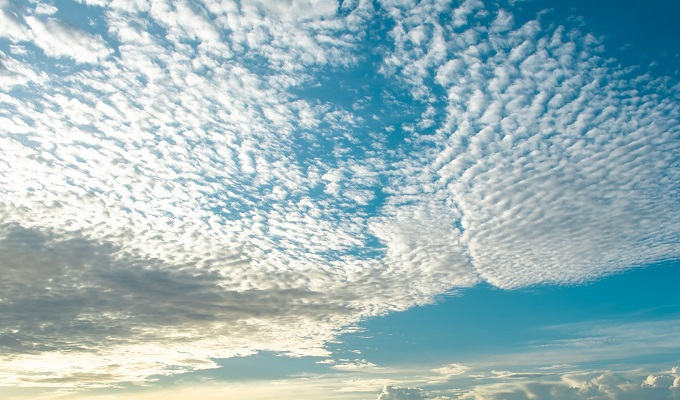
\includegraphics[width=6cm]{clouds/altocumulus.jpg}
    \caption{Altocumulus clouds \protect\cite{cloudtypes:wiki:altocumulus}.}
    \label{img:clouds:altocumulus}
\end{wrapfigure}
As with the cirrocumulus clouds, altocumulus clouds consist of small, puffy, white and grey \gls{cloudlet}s.
These \gls{cloudlet}s are usually slightly bigger than the ones of the cirrocumulus cloud.
It is easy to tell them apart, as the altocumulus \gls{cloudlet}s are usually more grey than white and are shaded on one side.
Altocumulus clouds can form through the dispersion of altostratus clouds or through \gls{convection} (see \sectionref{section:clouds:convection}).
\emptyline
\textbf{Interpretation:}
Usually, they are found in settled weather. They do not produce \gls{precipitation} that reaches the surface.